% Thesis template, using input commands for the chapters. If you want to use
% "import" for your chapters (to have relative includes of figures or other
% content), have a look at main_import.tex

% Compile this file with pdflatex

% A two-sided book
\documentclass[11pt,twoside]{book}

\usepackage{graphicx}

% This is only used for the example frontmatter
\usepackage{tabularx}

% To generate PDF hyperlinks (in blue)
\usepackage[pdfpagemode={UseOutlines},bookmarks=true,bookmarksopen=true,
bookmarksopenlevel=0,bookmarksnumbered=true,hypertexnames=false,
colorlinks,linkcolor={blue},citecolor={blue},urlcolor={red},
pdfstartview={FitV},unicode,breaklinks=true]{hyperref}

% Font related packages
\usepackage{textcomp}
\usepackage[T1]{fontenc}
\usepackage[utf8]{inputenc}

% Math font packages (add/replace by your favorites)
\usepackage{amsmath}
\usepackage{amssymb}
\usepackage{bm}
\usepackage{color}

% For postscript drawings (if you want to include them)
\usepackage{pstricks}

% For links and doi's
\usepackage{url}
\usepackage{doi}

% For references (you could also use biblatex)
\usepackage[square, numbers, comma, sort&compress]{natbib}

% Language / hyphenation
\usepackage[english]{babel}

% This sets the margins
\usepackage[top=2.5cm, left=1.75cm, right=1.75cm, bottom=2.0cm,%
bindingoffset=7.5mm, headheight=15pt, paper=b5paper]{geometry}

% Set the headers and footers for all pages. See the fancyhdr documentation if
% you want to change this.
\usepackage{fancyhdr}
\fancyhf{}
\fancyhead[LE,RO]{\bfseries\thepage}
\fancyhead[CE]{\bfseries\nouppercase{\rightmark}} % Section in the right on even pages
\fancyhead[CO]{\bfseries\nouppercase{\leftmark}} % Chapter in the left on odd pages

\fancypagestyle{plain}{%
\fancyhf{} % clear all header and footer fields
\renewcommand{\headrulewidth}{0pt}
\renewcommand{\footrulewidth}{0pt}}

% This command can be used to make sure new chapters start on the right page
\newcommand{\tclear}{\clearpage{\pagestyle{empty}\cleardoublepage}}

% Change these
\newcommand{\ttitle}{Another Thesis Template}
\newcommand{\tauthor}{John Doe}

% PDF meta-data
\hypersetup{urlcolor=blue, colorlinks=true}
\hypersetup{pdftitle=\ttitle}
\hypersetup{pdfsubject=}
\hypersetup{pdfauthor=\tauthor}
\hypersetup{pdfkeywords=}

% This defines a new environment "chapabstract" (chapter abstract)
\makeatletter
\newenvironment{chapabstract}
{\begin{center}\begin{minipage}{0.9\textwidth}}
{\end{minipage}\end{center}}
\makeatother

\begin{document}

\pagestyle{fancy}

\frontmatter

\thispagestyle{empty}

% This is (approximately) the template for the TUe

\begin{center}
  \vspace*{1cm}
  {\Huge \textbf{\ttitle}}

  \vspace{2.5cm}

  {\Large PROEFSCHRIFT}

  \vspace{2.5cm}

  \begin{minipage}{0.85\textwidth}
    \begin{sloppypar}
      ter verkrijging van de graad van doctor aan de Technische Universiteit
      Eindhoven, op gezag van de rector magnificus,
      prof.dr.ir.~F.P.T.~Baaijens, voor een commissie aangewezen door het
      College voor Promoties, in het openbaar te verdedigen op donderdag 12
      november 2015 om 16.00 uur
    \end{sloppypar}
  \end{minipage}

  \vspace{2cm}

  door

  \vspace{2cm}

  \tauthor

  \vspace{2cm}

  geboren te Amsterdam
\end{center}

\clearpage
\thispagestyle{empty}
\noindent Dit proefschrift is goedgekeurd door de promotoren en de
samenstelling van de promotiecommissie is als volgt:

\vspace{0.7cm}

\noindent
\begin{tabularx}{\textwidth}{@{}ll}
  voorzitter: & prof.dr. Piet \\
  1$^e$ promotor: & prof.dr. Kees \\
  copromotor: & dr.ir. Annelies \\
  leden: & prof.dr.ir. Henk \\
              & prof.dr. Jan \\
              & prof.dr. Gerrit\\
  adviseur: & Femke
\end{tabularx}

\vspace{7cm}

\noindent Het onderzoek of ontwerp dat in dit proefschrift wordt beschreven is uitgevoerd
in overeenstemming met de TU/e Gedragscode Wetenschapsbeoefening.

\clearpage

% Thanking some organization can be important to get the printing reimbursed!

\vspace*{4cm}
\noindent This research is supported by the Dutch Technology Foundation STW, which is part
of the Netherlands Organisation for Scientific Research (NWO) and partly funded
by the Ministry of Economic Affairs (project number XXXXX).

% Logo
% \begin{figure*}[!h]
%   \centering
%   \includegraphics[width=5cm]{STW-Ned-RGB.png}
% \end{figure*}


\tableofcontents

\tclear

\mainmatter

\chapter{This is a really long title, way too long to appear on top of this page}
\chaptermark{But this title is shorter}
\label{ch:long-chapter}

\begin{chapabstract}
  Lorem ipsum dolor sit amet, consectetur adipiscing elit. Donec a diam lectus.
  Sed sit amet ipsum mauris. Maecenas congue ligula ac quam viverra nec
  consectetur ante hendrerit. Donec et mollis dolor. Praesent et diam eget
  libero egestas mattis sit amet vitae augue. Nam tincidunt congue enim, ut
  porta lorem lacinia consectetur. Donec ut libero sed arcu vehicula ultricies a
  non tortor. Lorem ipsum dolor sit amet, consectetur adipiscing elit. Aenean ut
  gravida lorem. Ut turpis felis, pulvinar a semper sed, adipiscing id dolor.
  Pellentesque auctor nisi id magna consequat sagittis. Curabitur dapibus enim
  sit amet elit pharetra tincidunt feugiat nisl imperdiet. Ut convallis libero
  in urna ultrices accumsan. Donec sed odio eros. Donec viverra mi quis quam
  pulvinar at malesuada arcu rhoncus. Cum sociis natoque penatibus et magnis dis
  parturient montes, nascetur ridiculus mus. In rutrum accumsan ultricies.
  Mauris vitae nisi at sem facilisis semper ac in est.
\end{chapabstract}

\section{Hello}
\label{sec:ch1-hello}

Here are some citations:
\cite{Teunissen_thesis_2015,Teunissen_2014,Teunissen_2014b}, and some more:
\cite{Dubinova_2014,Nijdam_2014,Sun_2014,Sun_2013,Li_comparison_2012,Dhali_1985}.
And even more: \cite{Aleksandrov_1996,Allan_2006,Amestoy_2001}. Have a look at figure

\begin{figure}
  \centering
  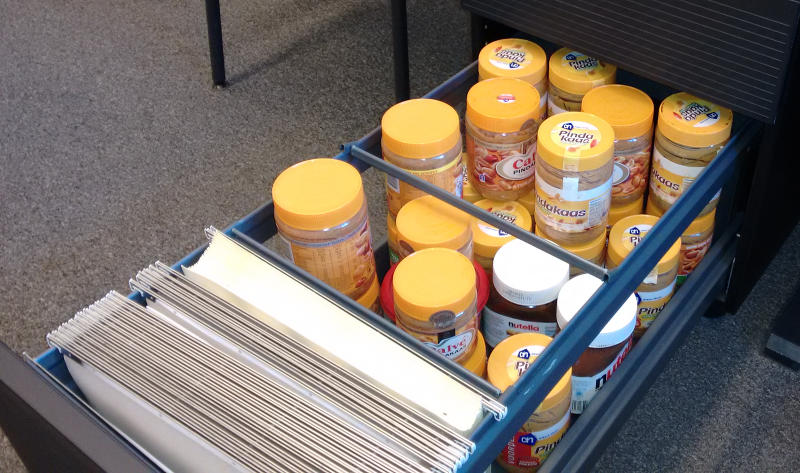
\includegraphics[width=0.7\textwidth]{figures/peanut_butter.jpg}
  \caption{Some people eat a lot of peanut butter}
  \label{fig:ch1-peanut-butter}
\end{figure}

Lorem ipsum dolor sit amet, consectetur adipiscing elit. Donec a diam lectus.
Sed sit amet ipsum mauris. Maecenas congue ligula ac quam viverra nec
consectetur ante hendrerit. Donec et mollis dolor. Praesent et diam eget libero
egestas mattis sit amet vitae augue. Nam tincidunt congue enim, ut porta lorem
lacinia consectetur. Donec ut libero sed arcu vehicula ultricies a non tortor.
Lorem ipsum dolor sit amet, consectetur adipiscing elit. Aenean ut gravida
lorem. Ut turpis felis, pulvinar a semper sed, adipiscing id dolor. Pellentesque
auctor nisi id magna consequat sagittis. Curabitur dapibus enim sit amet elit
pharetra tincidunt feugiat nisl imperdiet. Ut convallis libero in urna ultrices
accumsan. Donec sed odio eros. Donec viverra mi quis quam pulvinar at malesuada
arcu rhoncus. Cum sociis natoque penatibus et magnis dis parturient montes,
nascetur ridiculus mus. In rutrum accumsan ultricies. Mauris vitae nisi at sem
facilisis semper ac in est.

\section{Hello again}
\label{sec:ch1-hello-again}

Lorem ipsum dolor sit amet, consectetur adipiscing elit. Donec a diam lectus.
Sed sit amet ipsum mauris. Maecenas congue ligula ac quam viverra nec
consectetur ante hendrerit. Donec et mollis dolor. Praesent et diam eget libero
egestas mattis sit amet vitae augue. Nam tincidunt congue enim, ut porta lorem
lacinia consectetur. Donec ut libero sed arcu vehicula ultricies a non tortor.
Lorem ipsum dolor sit amet, consectetur adipiscing elit. Aenean ut gravida
lorem. Ut turpis felis, pulvinar a semper sed, adipiscing id dolor. Pellentesque
auctor nisi id magna consequat sagittis. Curabitur dapibus enim sit amet elit
pharetra tincidunt feugiat nisl imperdiet. Ut convallis libero in urna ultrices
accumsan. Donec sed odio eros. Donec viverra mi quis quam pulvinar at malesuada
arcu rhoncus. Cum sociis natoque penatibus et magnis dis parturient montes,
nascetur ridiculus mus. In rutrum accumsan ultricies. Mauris vitae nisi at sem
facilisis semper ac in est.

Lorem ipsum dolor sit amet, consectetur adipiscing elit. Donec a diam lectus.
Sed sit amet ipsum mauris. Maecenas congue ligula ac quam viverra nec
consectetur ante hendrerit. Donec et mollis dolor. Praesent et diam eget libero
egestas mattis sit amet vitae augue. Nam tincidunt congue enim, ut porta lorem
lacinia consectetur. Donec ut libero sed arcu vehicula ultricies a non tortor.
Lorem ipsum dolor sit amet, consectetur adipiscing elit. Aenean ut gravida
lorem. Ut turpis felis, pulvinar a semper sed, adipiscing id dolor. Pellentesque
auctor nisi id magna consequat sagittis. Curabitur dapibus enim sit amet elit
pharetra tincidunt feugiat nisl imperdiet. Ut convallis libero in urna ultrices
accumsan. Donec sed odio eros. Donec viverra mi quis quam pulvinar at malesuada
arcu rhoncus. Cum sociis natoque penatibus et magnis dis parturient montes,
nascetur ridiculus mus. In rutrum accumsan ultricies. Mauris vitae nisi at sem
facilisis semper ac in est.

Lorem ipsum dolor sit amet, consectetur adipiscing elit. Donec a diam lectus.
Sed sit amet ipsum mauris. Maecenas congue ligula ac quam viverra nec
consectetur ante hendrerit. Donec et mollis dolor. Praesent et diam eget libero
egestas mattis sit amet vitae augue. Nam tincidunt congue enim, ut porta lorem
lacinia consectetur. Donec ut libero sed arcu vehicula ultricies a non tortor.
Lorem ipsum dolor sit amet, consectetur adipiscing elit. Aenean ut gravida
lorem. Ut turpis felis, pulvinar a semper sed, adipiscing id dolor. Pellentesque
auctor nisi id magna consequat sagittis. Curabitur dapibus enim sit amet elit
pharetra tincidunt feugiat nisl imperdiet. Ut convallis libero in urna ultrices
accumsan. Donec sed odio eros. Donec viverra mi quis quam pulvinar at malesuada
arcu rhoncus. Cum sociis natoque penatibus et magnis dis parturient montes,
nascetur ridiculus mus. In rutrum accumsan ultricies. Mauris vitae nisi at sem
facilisis semper ac in est.

Lorem ipsum dolor sit amet, consectetur adipiscing elit. Donec a diam lectus.
Sed sit amet ipsum mauris. Maecenas congue ligula ac quam viverra nec
consectetur ante hendrerit. Donec et mollis dolor. Praesent et diam eget libero
egestas mattis sit amet vitae augue. Nam tincidunt congue enim, ut porta lorem
lacinia consectetur. Donec ut libero sed arcu vehicula ultricies a non tortor.
Lorem ipsum dolor sit amet, consectetur adipiscing elit. Aenean ut gravida
lorem. Ut turpis felis, pulvinar a semper sed, adipiscing id dolor. Pellentesque
auctor nisi id magna consequat sagittis. Curabitur dapibus enim sit amet elit
pharetra tincidunt feugiat nisl imperdiet. Ut convallis libero in urna ultrices
accumsan. Donec sed odio eros. Donec viverra mi quis quam pulvinar at malesuada
arcu rhoncus. Cum sociis natoque penatibus et magnis dis parturient montes,
nascetur ridiculus mus. In rutrum accumsan ultricies. Mauris vitae nisi at sem
facilisis semper ac in est.

Lorem ipsum dolor sit amet, consectetur adipiscing elit. Donec a diam lectus.
Sed sit amet ipsum mauris. Maecenas congue ligula ac quam viverra nec
consectetur ante hendrerit. Donec et mollis dolor. Praesent et diam eget libero
egestas mattis sit amet vitae augue. Nam tincidunt congue enim, ut porta lorem
lacinia consectetur. Donec ut libero sed arcu vehicula ultricies a non tortor.
Lorem ipsum dolor sit amet, consectetur adipiscing elit. Aenean ut gravida
lorem. Ut turpis felis, pulvinar a semper sed, adipiscing id dolor. Pellentesque
auctor nisi id magna consequat sagittis. Curabitur dapibus enim sit amet elit
pharetra tincidunt feugiat nisl imperdiet. Ut convallis libero in urna ultrices
accumsan. Donec sed odio eros. Donec viverra mi quis quam pulvinar at malesuada
arcu rhoncus. Cum sociis natoque penatibus et magnis dis parturient montes,
nascetur ridiculus mus. In rutrum accumsan ultricies. Mauris vitae nisi at sem
facilisis semper ac in est.

\tclear

\chapter{Another chapter}
\label{ch:another-chapter}

\begin{chapabstract}
  Lorem ipsum dolor sit amet, consectetur adipiscing elit. Donec a diam lectus.
  Sed sit amet ipsum mauris. Maecenas congue ligula ac quam viverra nec
  consectetur ante hendrerit. Donec et mollis dolor. Praesent et diam eget
  libero egestas mattis sit amet vitae augue. Nam tincidunt congue enim, ut
  porta lorem lacinia consectetur. Donec ut libero sed arcu vehicula ultricies a
  non tortor. Lorem ipsum dolor sit amet, consectetur adipiscing elit. Aenean ut
  gravida lorem. Ut turpis felis, pulvinar a semper sed, adipiscing id dolor.
  Pellentesque auctor nisi id magna consequat sagittis. Curabitur dapibus enim
  sit amet elit pharetra tincidunt feugiat nisl imperdiet. Ut convallis libero
  in urna ultrices accumsan. Donec sed odio eros. Donec viverra mi quis quam
  pulvinar at malesuada arcu rhoncus. Cum sociis natoque penatibus et magnis dis
  parturient montes, nascetur ridiculus mus. In rutrum accumsan ultricies.
  Mauris vitae nisi at sem facilisis semper ac in est.
\end{chapabstract}

\section{Hello}
\label{sec:ch2-hello}

Lorem ipsum dolor sit amet, consectetur adipiscing elit. Donec a diam lectus.
Sed sit amet ipsum mauris. Maecenas congue ligula ac quam viverra nec
consectetur ante hendrerit. Donec et mollis dolor. Praesent et diam eget libero
egestas mattis sit amet vitae augue. Nam tincidunt congue enim, ut porta lorem
lacinia consectetur. Donec ut libero sed arcu vehicula ultricies a non tortor.
Lorem ipsum dolor sit amet, consectetur adipiscing elit. Aenean ut gravida
lorem. Ut turpis felis, pulvinar a semper sed, adipiscing id dolor. Pellentesque
auctor nisi id magna consequat sagittis. Curabitur dapibus enim sit amet elit
pharetra tincidunt feugiat nisl imperdiet. Ut convallis libero in urna ultrices
accumsan. Donec sed odio eros. Donec viverra mi quis quam pulvinar at malesuada
arcu rhoncus. Cum sociis natoque penatibus et magnis dis parturient montes,
nascetur ridiculus mus. In rutrum accumsan ultricies. Mauris vitae nisi at sem
facilisis semper ac in est.

\section{Hello again}
\label{sec:ch2-hello-again}

Lorem ipsum dolor sit amet, consectetur adipiscing elit. Donec a diam lectus.
Sed sit amet ipsum mauris. Maecenas congue ligula ac quam viverra nec
consectetur ante hendrerit. Donec et mollis dolor. Praesent et diam eget libero
egestas mattis sit amet vitae augue. Nam tincidunt congue enim, ut porta lorem
lacinia consectetur. Donec ut libero sed arcu vehicula ultricies a non tortor.
Lorem ipsum dolor sit amet, consectetur adipiscing elit. Aenean ut gravida
lorem. Ut turpis felis, pulvinar a semper sed, adipiscing id dolor. Pellentesque
auctor nisi id magna consequat sagittis. Curabitur dapibus enim sit amet elit
pharetra tincidunt feugiat nisl imperdiet. Ut convallis libero in urna ultrices
accumsan. Donec sed odio eros. Donec viverra mi quis quam pulvinar at malesuada
arcu rhoncus. Cum sociis natoque penatibus et magnis dis parturient montes,
nascetur ridiculus mus. In rutrum accumsan ultricies. Mauris vitae nisi at sem
facilisis semper ac in est.

Lorem ipsum dolor sit amet, consectetur adipiscing elit. Donec a diam lectus.
Sed sit amet ipsum mauris. Maecenas congue ligula ac quam viverra nec
consectetur ante hendrerit. Donec et mollis dolor. Praesent et diam eget libero
egestas mattis sit amet vitae augue. Nam tincidunt congue enim, ut porta lorem
lacinia consectetur. Donec ut libero sed arcu vehicula ultricies a non tortor.
Lorem ipsum dolor sit amet, consectetur adipiscing elit. Aenean ut gravida
lorem. Ut turpis felis, pulvinar a semper sed, adipiscing id dolor. Pellentesque
auctor nisi id magna consequat sagittis. Curabitur dapibus enim sit amet elit
pharetra tincidunt feugiat nisl imperdiet. Ut convallis libero in urna ultrices
accumsan. Donec sed odio eros. Donec viverra mi quis quam pulvinar at malesuada
arcu rhoncus. Cum sociis natoque penatibus et magnis dis parturient montes,
nascetur ridiculus mus. In rutrum accumsan ultricies. Mauris vitae nisi at sem
facilisis semper ac in est.

\tclear

\addtocontents{toc}{\vspace{1em}} % Add a gap in the Contents, for aesthetics

\appendix

\chapter{An appendix}
\label{ch:appendix}

Lorem ipsum dolor sit amet, consectetur adipiscing elit. Donec a diam lectus.
Sed sit amet ipsum mauris. Maecenas congue ligula ac quam viverra nec
consectetur ante hendrerit. Donec et mollis dolor. Praesent et diam eget libero
egestas mattis sit amet vitae augue. Nam tincidunt congue enim, ut porta lorem
lacinia consectetur. Donec ut libero sed arcu vehicula ultricies a non tortor.
Lorem ipsum dolor sit amet, consectetur adipiscing elit. Aenean ut gravida
lorem. Ut turpis felis, pulvinar a semper sed, adipiscing id dolor. Pellentesque
auctor nisi id magna consequat sagittis. Curabitur dapibus enim sit amet elit
pharetra tincidunt feugiat nisl imperdiet. Ut convallis libero in urna ultrices
accumsan. Donec sed odio eros. Donec viverra mi quis quam pulvinar at malesuada
arcu rhoncus. Cum sociis natoque penatibus et magnis dis parturient montes,
nascetur ridiculus mus. In rutrum accumsan ultricies. Mauris vitae nisi at sem
facilisis semper ac in est.

Lorem ipsum dolor sit amet, consectetur adipiscing elit. Donec a diam lectus.
Sed sit amet ipsum mauris. Maecenas congue ligula ac quam viverra nec
consectetur ante hendrerit. Donec et mollis dolor. Praesent et diam eget libero
egestas mattis sit amet vitae augue. Nam tincidunt congue enim, ut porta lorem
lacinia consectetur. Donec ut libero sed arcu vehicula ultricies a non tortor.
Lorem ipsum dolor sit amet, consectetur adipiscing elit. Aenean ut gravida
lorem. Ut turpis felis, pulvinar a semper sed, adipiscing id dolor. Pellentesque
auctor nisi id magna consequat sagittis. Curabitur dapibus enim sit amet elit
pharetra tincidunt feugiat nisl imperdiet. Ut convallis libero in urna ultrices
accumsan. Donec sed odio eros. Donec viverra mi quis quam pulvinar at malesuada
arcu rhoncus. Cum sociis natoque penatibus et magnis dis parturient montes,
nascetur ridiculus mus. In rutrum accumsan ultricies. Mauris vitae nisi at sem
facilisis semper ac in est.

\tclear

\addtocontents{toc}{\vspace{1em}} % Add a gap in the Contents, for aesthetics

\backmatter

% This style file only shows doi's, no url's
\bibliographystyle{unsrtnat_nourl}
\bibliography{bib_example}

\chapter{Acknowledgements}
\label{ch:acknowledgements}

I would like to express my deepest gratitude to the Spaghetti Monster.



\tclear

\end{document}

